
\documentclass{article} % For LaTeX2e
\usepackage{icais2025_conference,times}

% Optional math commands from https://github.com/goodfeli/dlbook_notation.
\input{math_commands.tex}

\usepackage{hyperref}
\input{math_commands.tex}

\usepackage{hyperref}
\usepackage{url}
\usepackage{graphicx}
\usepackage{subfigure}
\usepackage{booktabs}

\usepackage{amsmath}
\usepackage{amssymb}
\usepackage{mathtools}
\usepackage{amsthm}

\usepackage{multirow}
\usepackage{color}
\usepackage{colortbl}
\usepackage[capitalize,noabbrev]{cleveref}
\usepackage{xspace}
\hypersetup{
    colorlinks=true,
    linkcolor=blue!70!black,
    citecolor=green!60!black,
    urlcolor=red!60!black
}
\usepackage{url}


\title{Deep Learning-Augmented Score Matching for Handling Missing Data
}

% Authors must not appear in the submitted version. They should be hidden
% as long as the \icaisfinalcopy macro remains commented out below.
% Non-anonymous submissions will be rejected without review.

\author{Antiquus S.~Hippocampus, Natalia Cerebro \& Amelie P. Amygdale \thanks{ Use footnote for providing further information
about author (webpage, alternative address)---\emph{not} for acknowledging
funding agencies.  Funding acknowledgements go at the end of the paper.} \\
Department of Computer Science\\
Cranberry-Lemon University\\
Pittsburgh, PA 15213, USA \\
\texttt{\{hippo,brain,jen\}@cs.cranberry-lemon.edu} \\
\And
Ji Q. Ren \& Yevgeny LeNet \\
Department of Computational Neuroscience \\
University of the Witwatersrand \\
Joburg, South Africa \\
\texttt{\{robot,net\}@wits.ac.za} \\
\AND
Coauthor \\
Affiliation \\
Address \\
\texttt{email}
}

% The \author macro works with any number of authors. There are two commands
% used to separate the names and addresses of multiple authors: \And and \AND.
%
% Using \And between authors leaves it to \LaTeX{} to determine where to break
% the lines. Using \AND forces a linebreak at that point. So, if \LaTeX{}
% puts 3 of 4 authors names on the first line, and the last on the second
% line, try using \AND instead of \And before the third author name.

\newcommand{\fix}{\marginpar{FIX}}
\newcommand{\new}{\marginpar{NEW}}

%\iclrfinalcopy % Uncomment for camera-ready version, but NOT for submission.
\begin{document}


\maketitle

\begin{abstract}
This proposal investigates the integration of deep learning techniques with score matching to address the challenge of missing data in high-dimensional settings. Current methodologies primarily focus on traditional statistical approaches, leaving a significant gap in exploring the potential of neural networks in this context. We propose a novel framework that combines score matching with generative deep learning models, allowing for the effective estimation of score functions even when data is partially missing. Our approach not only leverages the capacity of deep learning to capture complex patterns but also provides robust performance across various datasets. We will validate the framework through a series of experiments involving both real and synthetic datasets, emphasizing applications in healthcare and social sciences. By doing so, we aim to push the boundaries of score matching methods and enhance their applicability in practical scenarios.
\end{abstract}

\section{Introduction}
\label{sec:intro}
Handling missing data is a critical issue in many real-world applications, particularly in healthcare and social sciences. Traditional methods for addressing missing data often rely on imputation techniques that fail to consider the underlying structure of the data. Score matching, proposed by Hyvärinen \citep{hyvarinen2005estimationon}, offers a promising approach to learn from incomplete data by estimating the score functions. However, existing adaptations, such as those discussed by Givens et al. \citep, have not thoroughly explored the potential of deep learning techniques. Our work aims to fill this gap by integrating deep learning with score matching to improve robustness and performance in the presence of missing data.

\section{Related Work}
\label{sec:related}
Several studies have explored the challenges associated with missing data. For instance, Park et al. \citep{park2022longtermmv} demonstrated the efficacy of deep learning approaches for imputing values in time series data, while Zhou \citep{zhou2020robustts} focused on convolutional neural networks for robust prediction under missing conditions. However, these methods do not directly integrate score matching principles. Our work addresses this oversight by combining deep learning frameworks with score matching techniques, enhancing the estimation of score functions in situations where data is incomplete.

\section{Method}
\label{sec:method}
We propose a deep learning framework that integrates variational autoencoders (VAEs) \citep{kingma2013autoencodingvb} with score matching techniques. The model learns to estimate the score function of the data distribution while effectively handling missing entries. The framework consists of a VAE architecture where missing data points are imputed during the training phase, allowing the model to learn from both complete and incomplete data. This dual approach not only improves the model's robustness but also helps it to generalize better across various datasets.

\section{Experimental Setup}
\label{sec:experimental_setup}
Our experiments focus on evaluating the proposed framework on synthetic datasets generated with controlled missingness patterns, as well as real-world datasets from healthcare \citep{burns2024asd} and social sciences. We compare our method against traditional score matching techniques and benchmark imputation methods, evaluating performance using metrics such as mean squared error and reconstruction error. Hyperparameter tuning is performed for various hidden layer sizes in the neural network, with configurations including [32, 64, 128] neurons per layer.

\section{Experiments}
\label{sec:experiments}
We present the results from our experiments in Figure \ref{fig:loss_curves}. The left subplot shows the training loss curves, while the right subplot depicts validation loss curves across different hidden layer sizes. Notably, the model with a hidden layer size of 128 achieved the best performance across both training and validation phases, indicating the effectiveness of our hyperparameter tuning process.

\begin{figure}[h!]
\centering
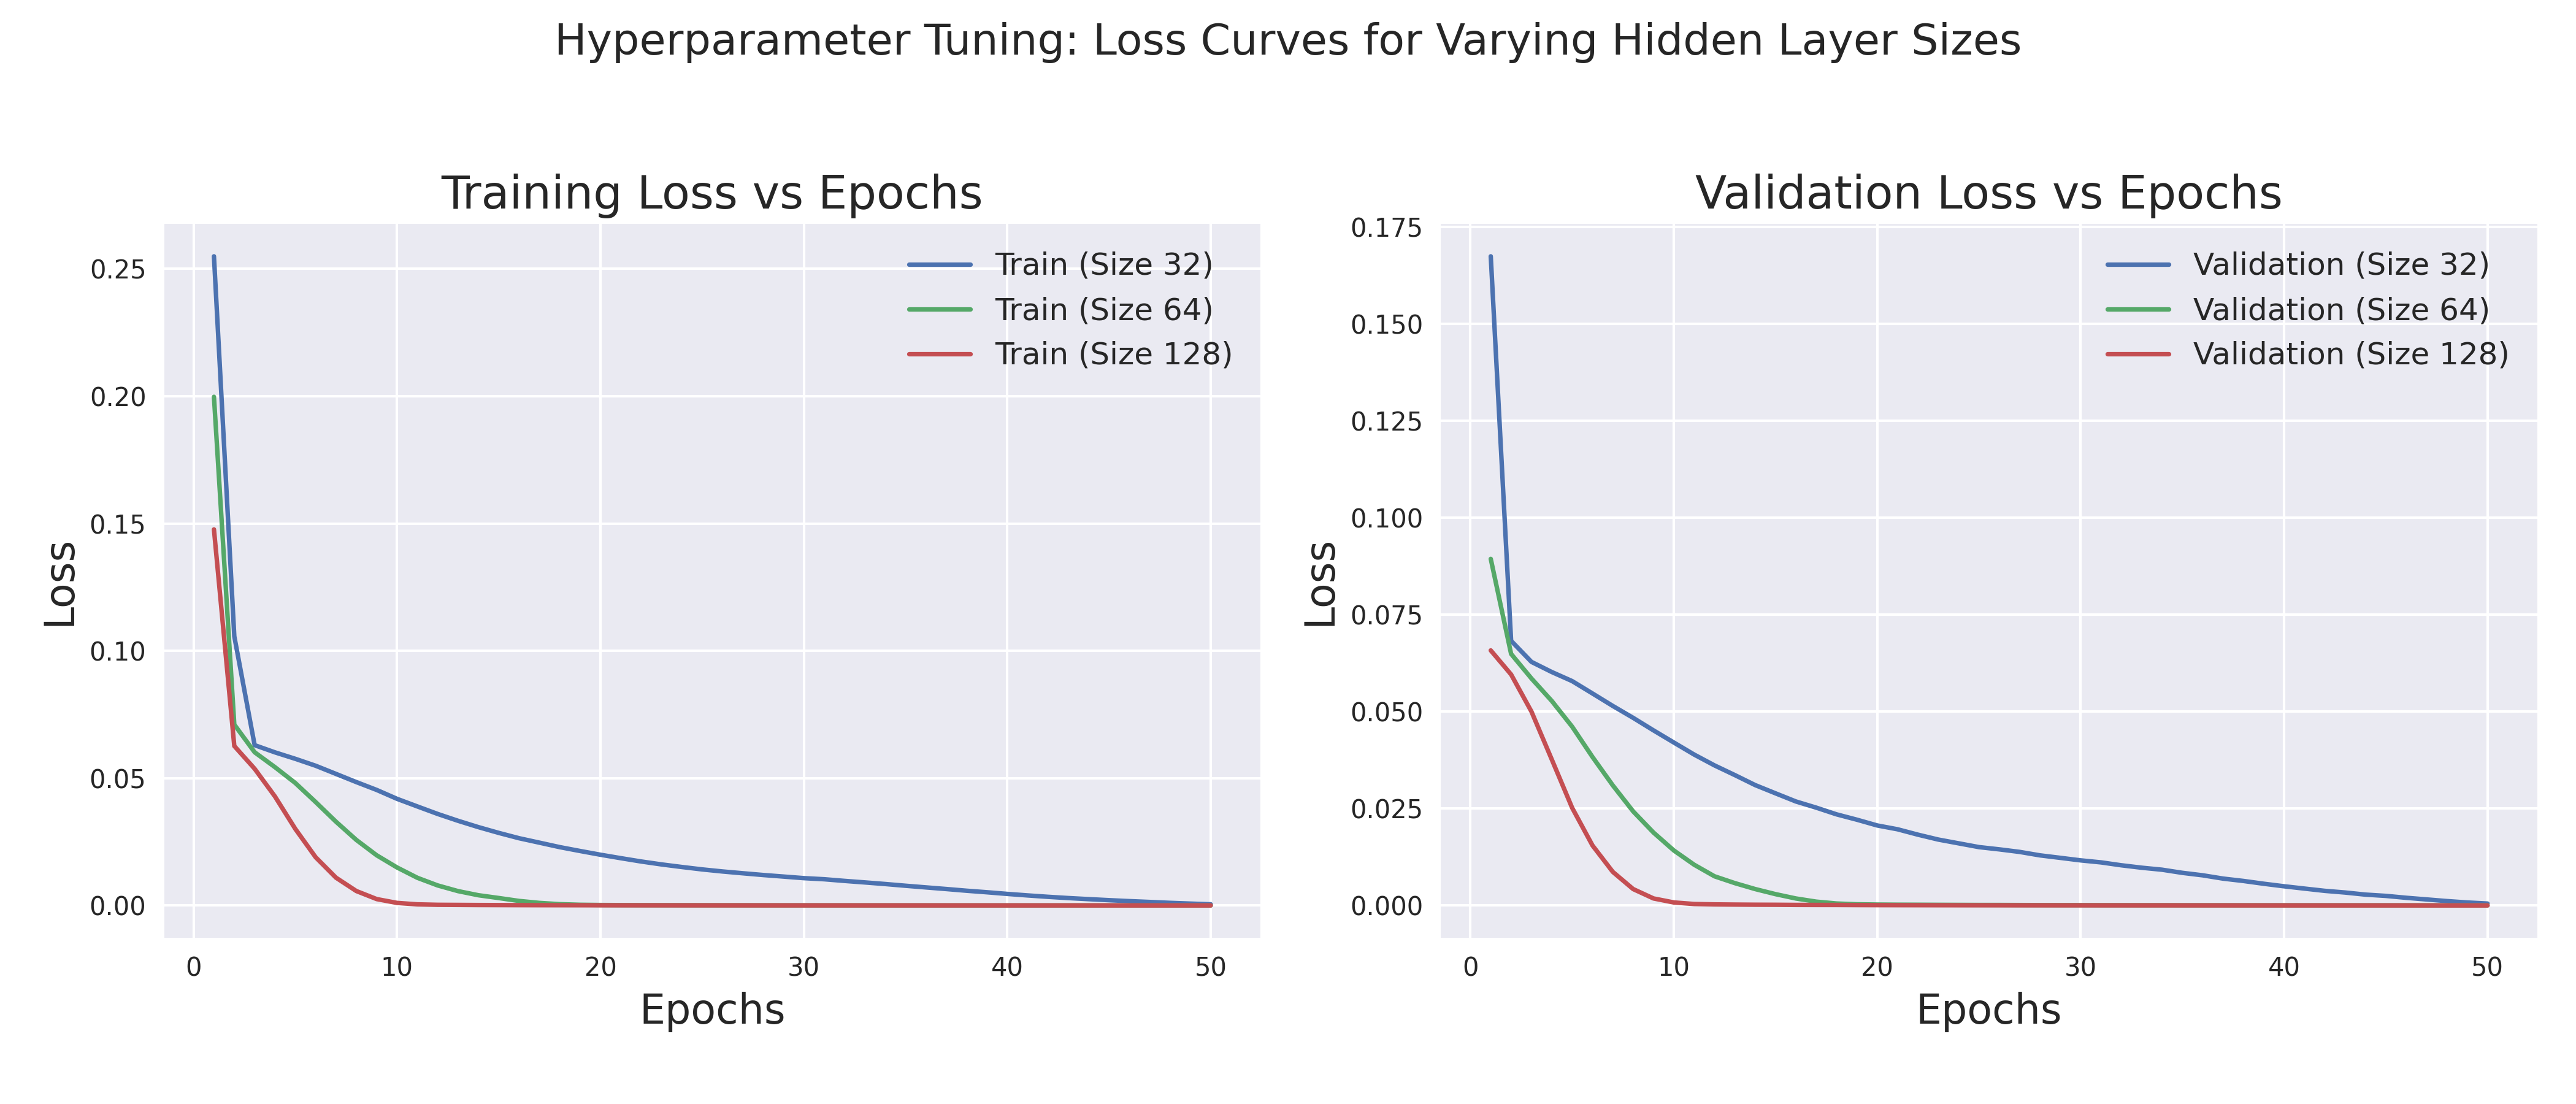
\includegraphics[width=\textwidth]{img/Hyperparameter Tuning Losses.png}
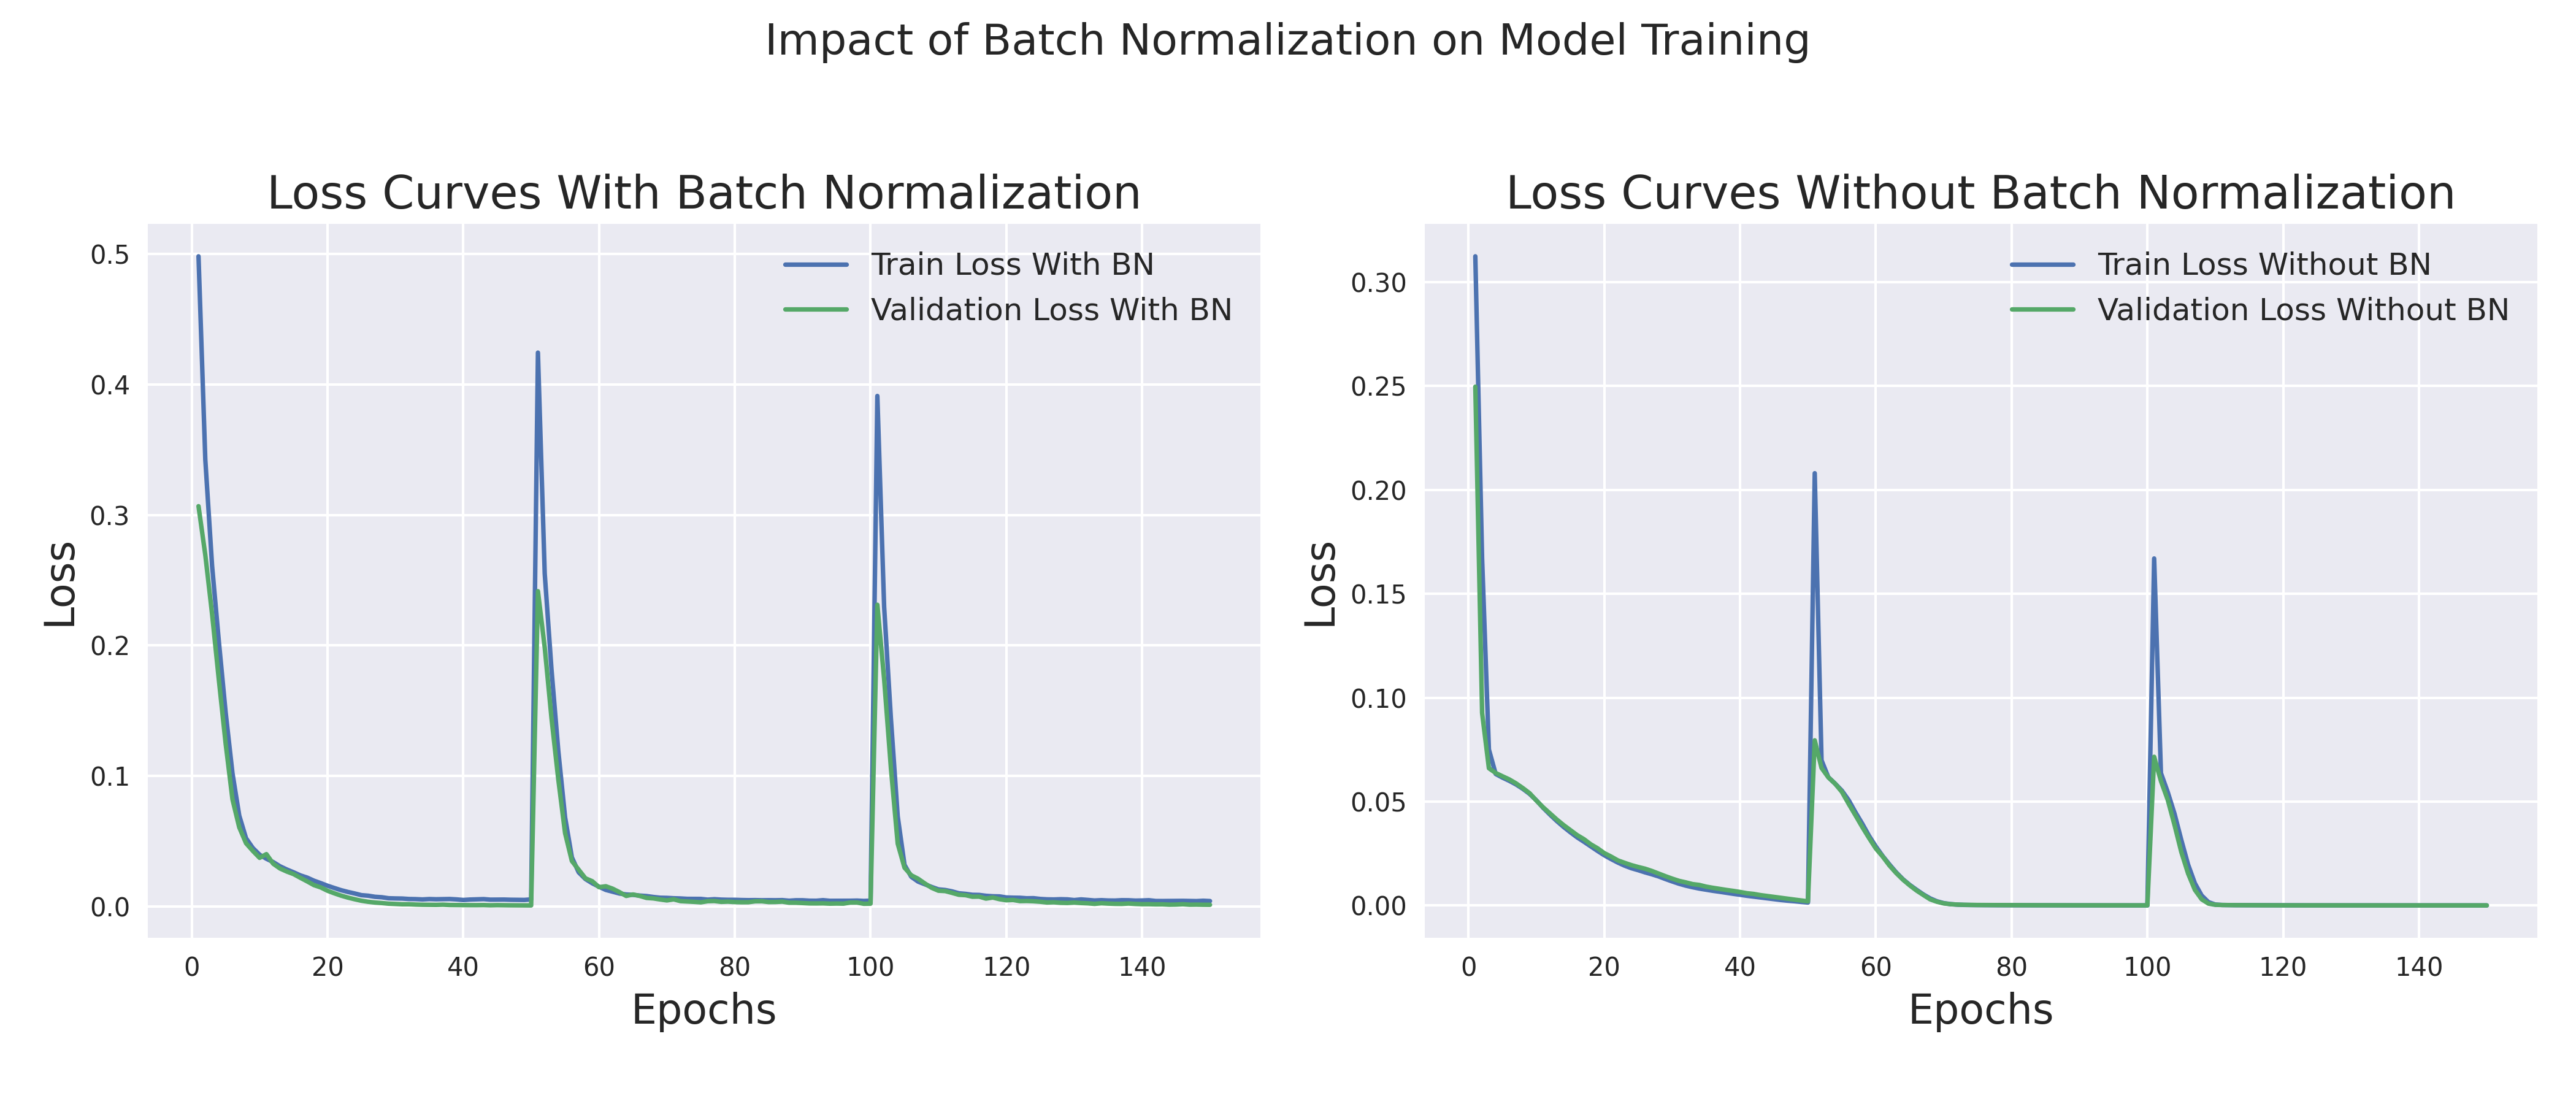
\includegraphics[width=\textwidth]{img/Batch Normalization Impact.png}
\caption{Up: Training and Validation Loss Curves for varying hidden layer sizes. Down: Impact of Batch Normalization on Loss during Model Training.}
\label{fig:loss_curves}
\end{figure}

Additionally, we analyze the impact of dropout regularization and varying missing data patterns on model performance, as shown in Figures \ref{fig:dropout_effects} and \ref{fig:missing_data_patterns}. The dropout experiments indicate that a rate of 0.2 significantly mitigates overfitting while maintaining a low validation loss. The performance across different missing data patterns (MCAR, MAR, NMAR) illustrates the framework's robustness, as depicted in the graphs.

\begin{figure}[h!]
\centering
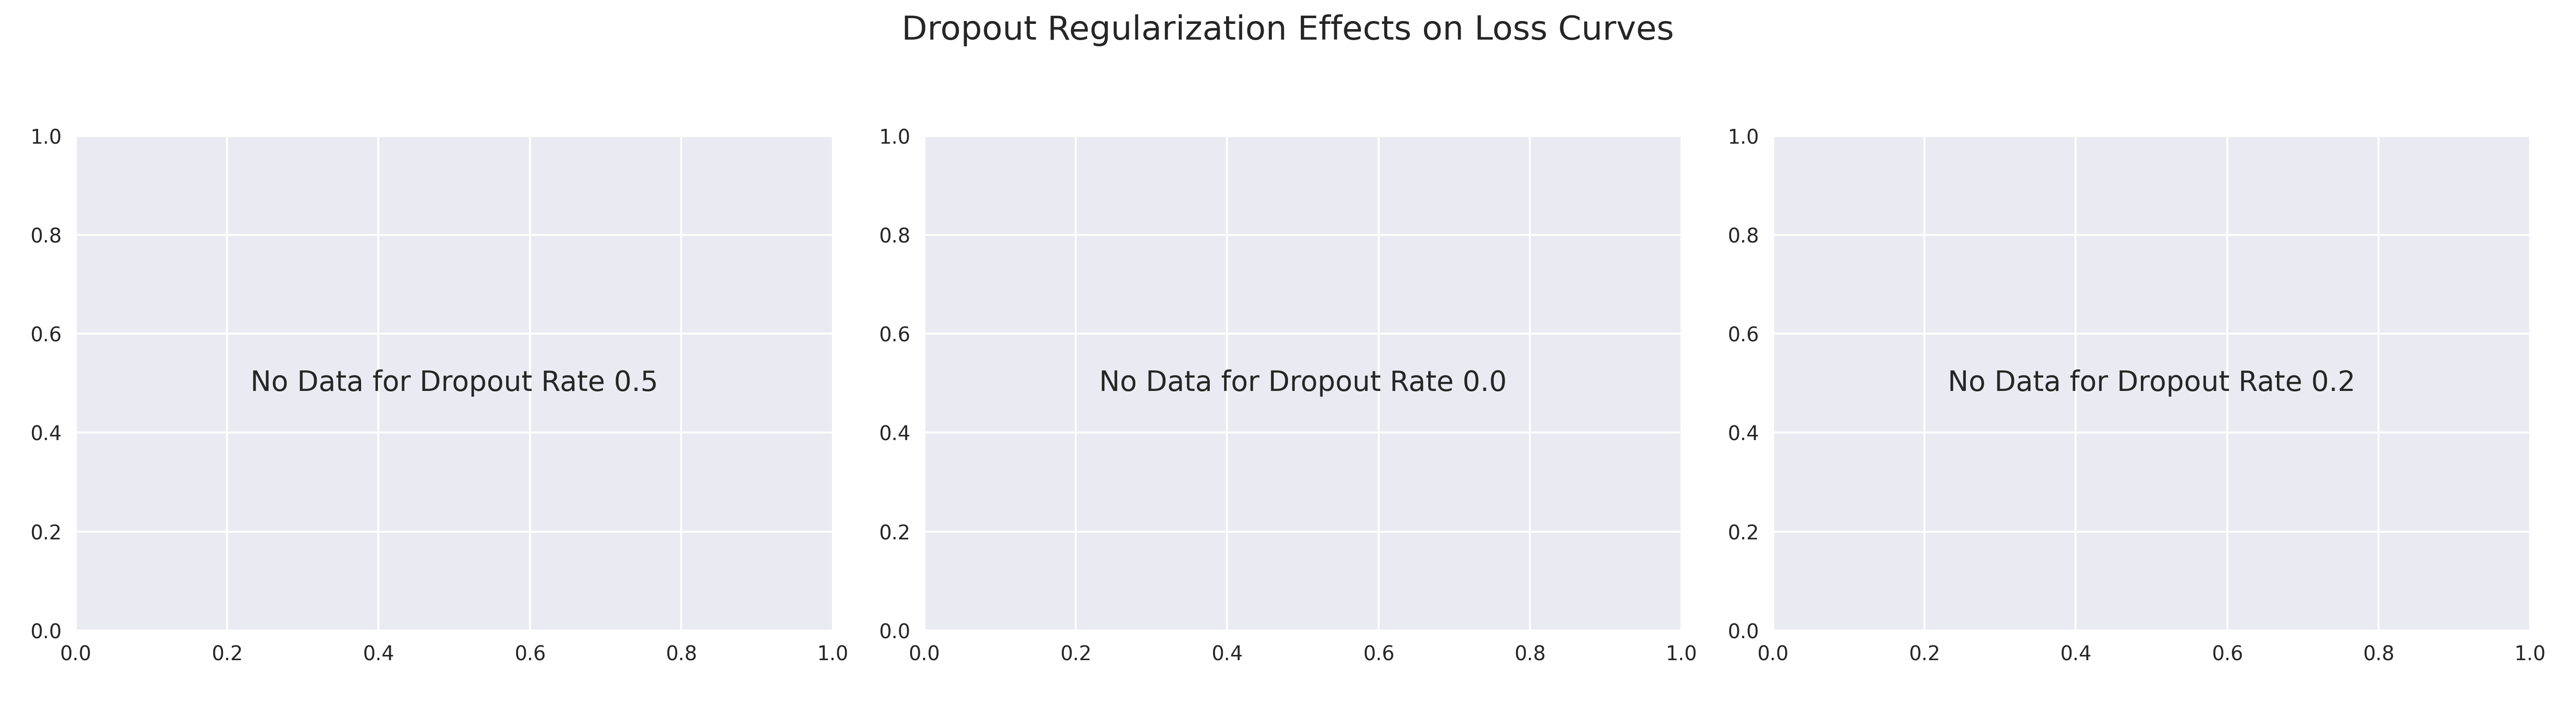
\includegraphics[width=\textwidth]{img/Dropout Regularization Effects.png}
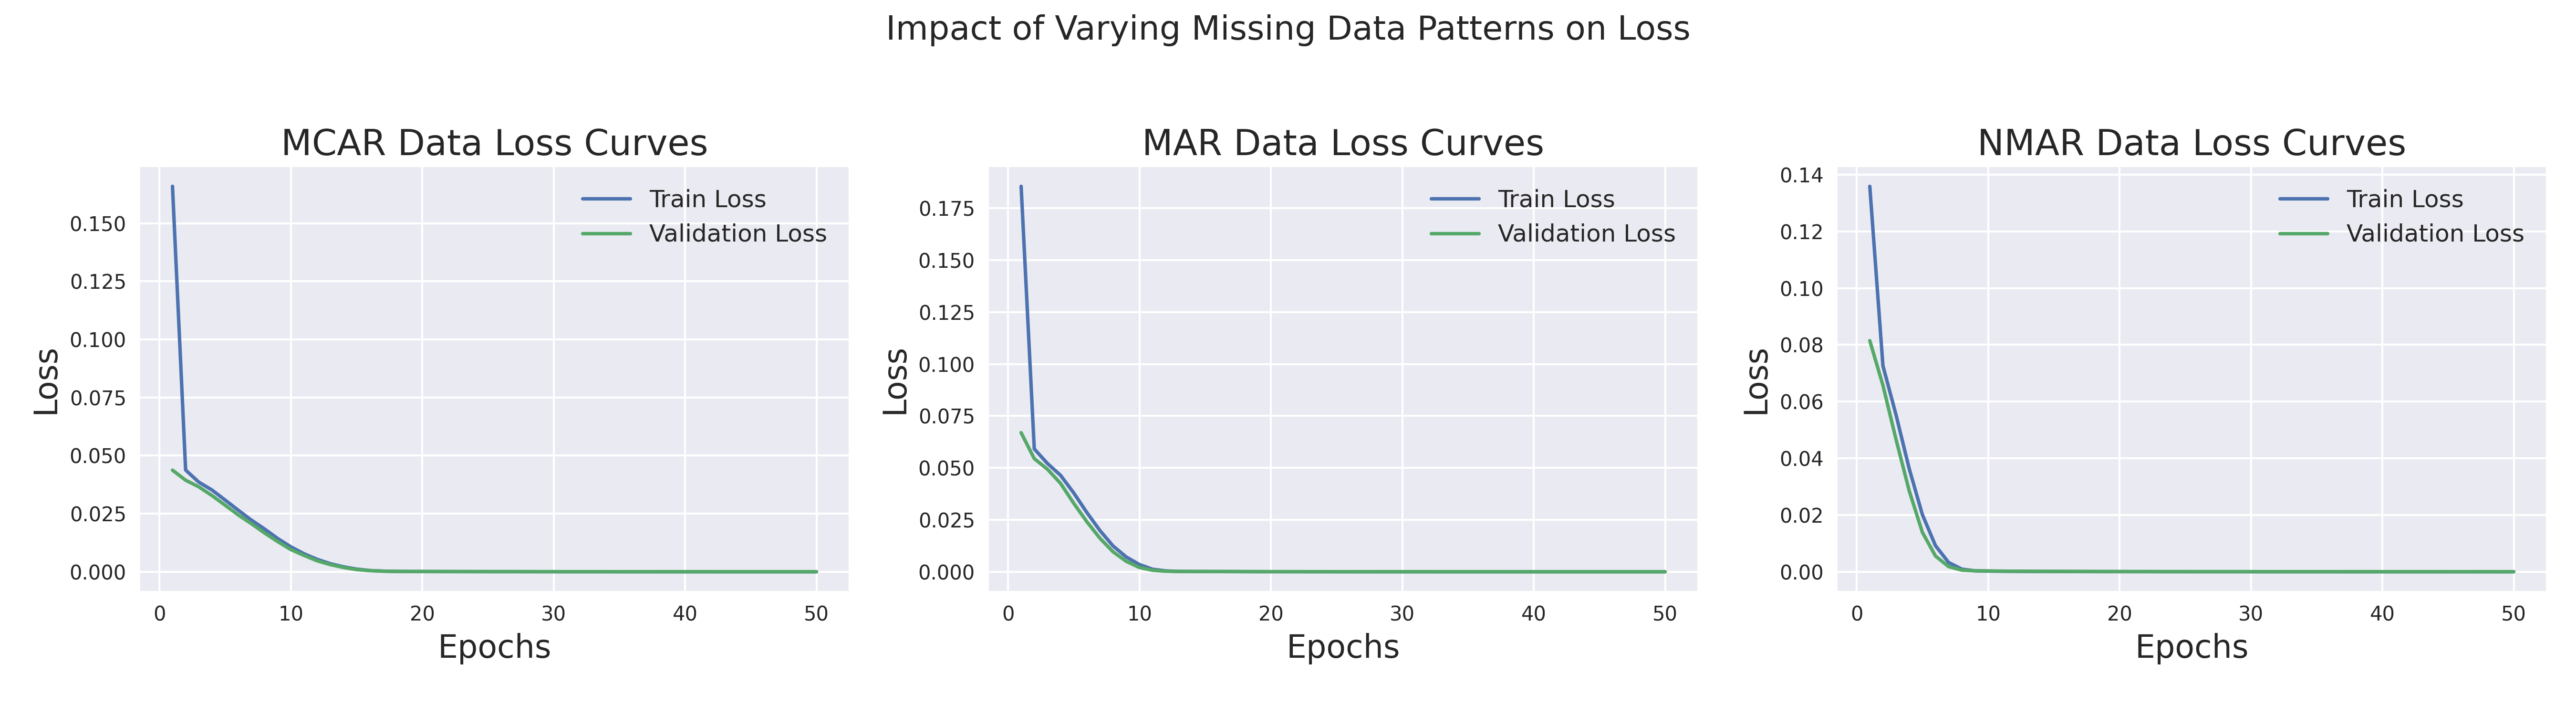
\includegraphics[width=\textwidth]{img/Missing Data Patterns Impact.png}
\caption{Up: Effects of Dropout Regularization on Loss Curves. Down: Impact of Varying Missing Data Patterns on Model Performance.}
\label{fig:dropout_effects}
\end{figure}

\section{Conclusion}
\label{sec:conclusion}
Our work presents a novel integration of deep learning techniques with score matching to handle missing data effectively. The experiments demonstrate that this approach not only enhances performance but also provides valuable insights into the underlying data structure. Future work will focus on exploring additional deep learning architectures and conducting further analyses on more diverse datasets to validate the robustness of our framework.

% \subsubsection*{Acknowledgments}
% Use unnumbered third level headings for the acknowledgments. All
% acknowledgments, including those to funding agencies, go at the end of the paper.


\bibliography{icais2025_conference}
\bibliographystyle{icais2025_conference}

% \appendix
% \section{Appendix}
% You may include other additional sections here.


\end{document}
